\documentclass[a4paper,10pt,twocolumn]{article}

\usepackage{amsmath}
\usepackage{amssymb}
\usepackage[english]{babel}
\usepackage[style=ieee,backend=bibtex]{biblatex}
	\bibliography{references.bib}
\usepackage{booktabs}
\usepackage[font={small},labelfont=sc]{caption}
\usepackage{helvet}
\usepackage[hidelinks]{hyperref}
\usepackage{fancyhdr}
\usepackage{float}
\usepackage[symbol]{footmisc}
\usepackage[margin=1in]{geometry}
\usepackage{graphicx}
\usepackage[latin1]{inputenc}
\usepackage{listings}
\usepackage{mathtools}
\usepackage{microtype}
\usepackage{multirow}
\usepackage{nomencl}
	\setlength{\nomitemsep}{0pt}
	\makenomenclature
\usepackage{rotating}
\usepackage{siunitx}
\usepackage{subcaption}
\usepackage{threeparttable}
\usepackage{tikz,pgfplots}
    \pgfplotsset{compat=1.15,set layers}
	\usetikzlibrary{angles}
	\usetikzlibrary{calc}
    \usetikzlibrary{external}
    	\tikzexternalize[prefix=tikz/]
	\usetikzlibrary{pgfplots.groupplots}
	\usetikzlibrary{positioning}
	\usetikzlibrary{shapes.misc}
    \usepgfplotslibrary{fillbetween}
\usepackage{titling}
\usepackage{xspace}

\renewcommand{\sfdefault}{phv}
\renewcommand{\familydefault}{\sfdefault}

\newcommand{\Matlab}{\textsc{Matlab}\textsuperscript{\textregistered}\xspace}
\newcommand{\sisotool}{\texttt{sisotool()}\xspace}
\newcommand{\sse}{\textsc{sse}\xspace}
\newcommand{\Sse}{\textsc{Sse}\xspace}

\title{Controller Design in \Matlab}
\author{Russell Maguire}
\date{\today}

\pagestyle{fancy}
\fancyhf{}
\lhead{
\includegraphics[width=0.1\textwidth]{img/Durham.png}}
\chead{\thetitle}
\rhead{\theauthor}
\cfoot{\thepage}

% Listings preamble
\definecolor{codegreen}{rgb}{0,0.6,0}
\definecolor{codegray}{rgb}{0.5,0.5,0.5}
\definecolor{codepurple}{rgb}{0.58,0,0.82}
\definecolor{backcolour}{rgb}{0.95,0.95,0.92}

\lstdefinestyle{mystyle}{
    backgroundcolor=\color{backcolour},
    commentstyle=\color{codegreen},
    keywordstyle=\color{magenta},
    numberstyle=\tiny\color{codegray},
    stringstyle=\color{codepurple},
    basicstyle=\ttfamily\small,
    breakatwhitespace=false,
    breaklines=true,
    captionpos=b,
    keepspaces=true,
    numbers=left,
    numbersep=5pt,
    showspaces=false,
    showstringspaces=false,
    showtabs=false,
    tabsize=2
}

\renewcommand{\thefootnote}{\fnsymbol{footnote}}

\begin{document}

% Title page.
% \begin{titlepage}
%     \centering
%     \vspace*{\fill}
%     
\includegraphics[width=0.5\textwidth]{img/Durham.png}\\
%     \vspace*{\fill}
%     \LARGE\thetitle\\
%     \vskip0.2em
%     \large Level 3 Control and Signal Processing\\
%     \vskip0.4em
%     \large\theauthor\\
%     \vskip0.4em
%     \large\thedate\\
%     \vspace*{\fill}
% \end{titlepage}

% Abstract
\twocolumn[{%
\begin{@twocolumnfalse} \centering
    \renewcommand{\abstractname}{\large Abstract}
    \vspace{-3\parsep}
    \begin{abstract}
        This report describes the design and characteristics of P, PD, PID and phase-lead controllers for an type I, III order industrial plant process in \Matlab. Controllers were designed to meet one of two performance specifications. After comparison it was concluded that PD controllers achieved the best performance.
    \end{abstract}
    \vspace{\parsep}
\end{@twocolumnfalse}
}]

% Acronyms
% Lowercase latin
\nomenclature[1e]{$e(\infty)$}{Steady state error\hfill[\si{\%}]}
\nomenclature[1s]{$s$}{Laplace domain variable\hfill[\si{\radian\per\second}]}
\nomenclature[1pc]{$p$}{Pole in Laplace domain\hfill[\si{\radian\per\second}]}
\nomenclature[1t]{$t$}{Time domain variable\hfill[\si{\second}]}
\nomenclature[1zc]{$z$}{Zero in Laplace domain\hfill[\si{\radian\per\second}]}

% Lowercase greek
\nomenclature[2f]{$\zeta$}{Damping factor}
\nomenclature[2z]{$\omega_n$}{Natural frequency\hfill[\si{\radian\per\second}]}

% Uppercase latin
\nomenclature[4G]{$G$}{Plant process transfer function}
\nomenclature[4Gc]{$G_c$}{Controller transfer function}
\nomenclature[4K]{$K$}{Plant process gain factor}
\nomenclature[4Kd]{$K_c$}{Controller gain factor}
\nomenclature[4Kd]{$K_d$}{Derivative gain factor}
\nomenclature[4Ki]{$K_i$}{Integral gain factor}
\nomenclature[4Kp]{$K_p$}{Proportional gain factor}
\nomenclature[4M0]{$M_0$}{Peak overshoot\hfill[\si{\%}]}
\nomenclature[4Td]{$T_d$}{Derivative time constant\hfill[\si{\second}]}
\nomenclature[4Ti]{$T_i$}{Integral time constant\hfill[\si{\second}]}
\nomenclature[4Tr]{$T_r$}{Rise time (\SIrange{10}{90}{\%})\hfill[\si{\second}]}
\nomenclature[4Ts]{$T_s$}{Settling time (\SI{2}{\%})\hfill[\si{\second}]}

% Uppercase greek
\begin{small}
	\printnomenclature
\end{small}

\section{Introduction}

Control systems find applications across engineering, economics and the environment.

Robotics are the obvious application where servo and stepper-motors are used in control systems to actuate precise armature movement.

Robots mimic control systems found in nature, such as the feedback between motor and sensory neurons in animals.

Many markets trade automatically, employing algorithms originally developed for electronic control theory.

\section{Background}

Figure~\ref{fig:closed} illustrates a closed loop system. The controller is designed to drive the output $y(s)$ of the plant process to the desired output $r(s)$ by minimising the error $e(s)$.

\begin{figure}[h!]
	\centering
	\small
	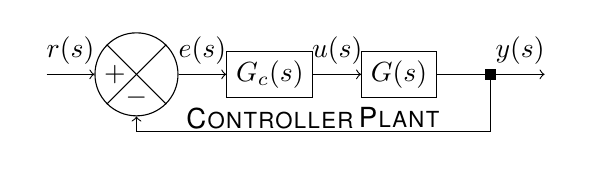
\begin{tikzpicture}[node distance=0.05\textwidth and 0.05\textwidth]
		\node (desire) {};
		\node [draw,right=of desire,circle,minimum size=3em] (sum) {};
			\draw (sum.north west) -- (sum.south east);
			\draw (sum.north east) -- (sum.south west);
		\node [draw,right=of sum,rectangle] (controller) {$G_c(s)$};
		\node [draw,right=of controller,rectangle] (plant) {$G(s)$};
		\node [fill,right=of plant,rectangle,inner sep=2pt] (branch) {};
		\node [right=of branch] (output) {};
		\node [below=of branch.center] (feedback1) {};
		\node [below=of sum.center] (feedback2) {};

		\draw [->] (desire) -- (sum);
		\draw [->] (sum) -- (controller);
		\draw [->] (controller) -- (plant);
		\draw [->] (plant) -- (output);
		\draw [->] (branch) -- (feedback1.center) -- (feedback2.center) -- (sum);

		\node [anchor=west] at (sum.west) {$+$};
		\node [anchor=south] at (sum.south) {$-$};

		\node [anchor=south west] at (desire) {$r(s)$};
		\node [anchor=south] at ($(sum.east)!0.5!(controller.west)$) {$e(s)$};
		\node [anchor=south] at ($(controller.east)!0.5!(plant.west)$) {$u(s)$};
		\node [anchor=south east] at (output) {$y(s)$};

		\node [anchor=north] at (controller.south) {\textsc{Controller}};
		\node [anchor=north] at (plant.south) {\textsc{Plant}};
	\end{tikzpicture}
	\caption{Block diagram of the closed loop system.}
	\label{fig:closed}
\end{figure}

The controller gain factor $K_c$ is a key design parameter and its effect on the system poles can be represented by the root locus. Each point on the root locus satisfies the angle criterion:
\begin{equation} \label{eq:angle} \textstyle % For the smaller \sum symbols
	\sum_i\angle\left(s-p_i\right) -\sum_j\angle\left(s-z_j\right) \equiv \pi \mod 2\pi
\end{equation}
This allows the root locus to be manipulated deterministically by adding poles and/or zeros. The controller gain at a point on the root locus can be determined using the magnitude criterion:
\begin{equation} \label{eq:magnitude}
	K_c\cdot K \equiv \frac{\prod_i\left|s-p_i\right|}{\prod_j\left|s-z_j\right|}
\end{equation}
where $K$ is the gain factor of the plant process transfer function.

\subsection{Performance}

For low frequency applications the controller performance can be characterised by analysing the step response.

Overshoot $M_0$ is the the peak response in proportion to the final output value and is soley dependent on the damping factor $\zeta$ for second order systems:
\begin{equation} \label{eq:overshoot2nd}
	M_0 = \exp\left(-\frac{\pi\zeta}{\sqrt{1-\zeta^2}}\right)
	\footnote{Equality holds for second order systems only, but may be used to approximate higher order characteristics.}
\end{equation}
The settling time $T_s$ of the controller is the time for the output oscillations to decay to within some margin of the final value: \SI{2}{\%} is used in this report. Settling time is also dependent on the natural frequency $\omega_n$:
\begin{equation} \label{eq:settling2nd}
	T_s = -\frac{\ln\left(2\%\right)}{\zeta\omega_n} \approx \frac{4}{\zeta\omega_n}
	\footnotemark[\value{footnote}]
\end{equation}
The rise time $T_r$ of the controller is the time for the output to transition from \SIrange{10}{90}{\%} of the final value:
\begin{equation} \label{eq:rise2nd}
	T_r = \frac{\ln\left(90\%/10\%\right)}{\zeta\omega_n} \approx \frac{2.2}{\zeta\omega_n}
	\footnotemark[\value{footnote}]
\end{equation}
These three parameters are typically specified as upper bounds and constitute the dynamic specification.

The steady state error $e(\infty)$ for a step input is defined and determined as follows:
\begin{align}
	e(\infty) \coloneqq& \lim_{t \rightarrow \infty}e(t) \label{eq:sse_def} \\
	=&
	\begin{cases} \displaystyle 
		\frac{1}{\displaystyle 1 + \lim_{s \rightarrow +0}G_c(s)G(s)}, &\operatorname{type}~0 \\
		0, &\operatorname{otherwise}
	\end{cases} \label{eq:sse}
\end{align}
where the type of the open loop transfer function $G_c(s)G(s)$ is the number of poles at the origin.

In controller design there is a tradeoff between the dynamic specification and the steady state error. The type of controller has a large impact on how the tradeoff is done.

\subsection{PID Control}

One of the most common types of controller in industry is the PID controller, which can be easily implemented using microcontrollers. Figure~\ref{fig:pid} shows how a PID controller is composed.

\begin{figure}[h!]
	\centering
	\small
	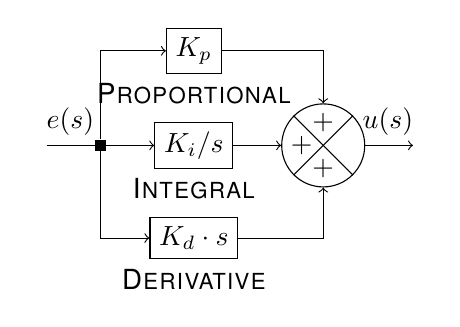
\begin{tikzpicture}[node distance=0.05\textwidth and 0.05\textwidth]
		\node (error) {};
		\node [fill,right=of error,rectangle,inner sep=2pt] (branch) {};
		\node [draw,right=of branch,rectangle] (i) {${K_i}/{s}$};
		\node [draw,above=of i,rectangle] (p) {$K_p$};
		\node [draw,below=of i,rectangle] (d) {${K_d}\cdot{s}$};
		\node [draw,right=of i,circle,minimum size=3em] (sum) {};
			\draw (sum.north west) -- (sum.south east);
			\draw (sum.north east) -- (sum.south west);
		\node [right=of sum] (output) {};

		\draw [->] (branch) |- (p);
		\draw [->] (error) -- (i);
		\draw [->] (branch) |- (d);
		\draw [->] (p) -| (sum);
		\draw [->] (i) -- (sum);
		\draw [->] (d) -| (sum);
		\draw [->] (sum) -- (output);

		\node [anchor=north] at (sum.north) {$+$};
		\node [anchor=west] at (sum.west) {$+$};
		\node [anchor=south] at (sum.south) {$+$};

		\node [anchor=south west] at (error) {$e(s)$};
		\node [anchor=south east] at (output) {$u(s)$};

		\node [anchor=north] at (p.south) {\textsc{Proportional}};
		\node [anchor=north] at (i.south) {\textsc{Integral}};
		\node [anchor=north] at (d.south) {\textsc{Derivative}};
	\end{tikzpicture}
	\caption{Block diagram of a PID controller}
	\label{fig:pid}
\end{figure}

The relative contribution of the derivative factor $K_d$ and intergral factor $K_i$ can be expressed as time constants $T_d$ and $T_i$ as follows:
\begin{align} \label{eq:T_i}
	T_i &= \frac{K_p}{K_i} & T_d &= \frac{K_d}{K_p}
\end{align}

Consequently, an equivalent form of the controller in Figure~\ref{fig:pid} is as follows:
\begin{equation}
	G_c(s) = K_p\left(1 + \frac{1}{T_i \cdot s} + T_d \cdot s\right)
\end{equation}

In any controller, the proportional gain $K_p$ is used to set the tradeoff between overshoot and speed. A faster system has a short rise and settling time but greater overshoot, achieved with a larger gain.

Increasing the contribution of the integrator term improves the steady-state performance at the expense of the dynamic performance. Generally, controllers with short $T_i$ have greater overshoot, longer rise and settling time but smaller steady-state error.

Increasing the contribution of the differentiator term improves the dynamic performance at the expense of the steady-state performance. Generally, controllers with large $T_d$ have smaller overshoot, shorter rise and settling time but greater steady-state error.

Some variations of the PID controller are named as follows:
\begin{itemize} \itemsep0pt
	\item \textbf{P controller} where $K_i$ and $K_d$ are zero. Also known as gain compensation.
	\item \textbf{PI controller} where $K_d$ is zero.
	\item \textbf{PD controller} where $K_i$ is zero. Used in 
\end{itemize}

\subsection{Phase Compensation}

Practical phase compensation involves adding real pole-zero pairs close to the origin to improve steady-state performance (phase-lag compensation) or left of the uncompensated root locus to improve dynamic peformance (phase-lead compensation) or both (lag-lead compenation). Figure~\ref{fig:phase} illustrates the block diagram of the compensator.

\begin{figure}[h!]
	\centering
	\small
	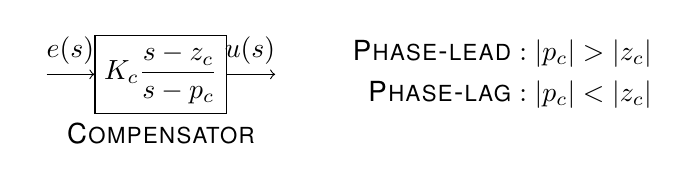
\begin{tikzpicture}[node distance=0.05\textwidth and 0.05\textwidth]
		\node (error) {};
		\node [draw,right=of error,rectangle] (C) {$K_c\dfrac{s-z_c}{s-p_c}$};
		\node [right=of C] (output) {};

		\draw [->] (error) -- (C);
		\draw [->] (C) -- (output);

		\node [anchor=south west] at (error) {$e(s)$};
		\node [anchor=south east] at (output) {$u(s)$};
		\node [right=of output] {$
			\begin{aligned}
				\textsc{Phase-lead}&: |p_c| > |z_c| \\
				\textsc{Phase-lag}&: |p_c| < |z_c|
			\end{aligned}
		$};

		\node [anchor=north] at (C.south) {\textsc{Compensator}};
	\end{tikzpicture}
	\caption{Block diagram of a phase-lead controller.}
	\label{fig:phase}
\end{figure}

The compensator gain $K_c$ is then used to tradeoff the overshoot and speed of the modified system, much like gain compensation.

\section{Specification}

The transfer function for the industrial plant process $G(s)$ was given as follows:
\begin{equation} \label{eq:G}
	G(s) = \frac{s + 1}{s(s^2 + 4s + 5)}
\end{equation}
The controller transfer functions $G_c(s)$ were chosen to meet the system performance specification detailed in Table~\ref{tab:spec}.

\begin{table}[h!]
	\centering
	\footnotesize
	\begin{threeparttable}
		\caption{System perfomance specification.}
		\label{tab:spec}
		\begin{tabular}{@{}crrrr@{}}
			\toprule
			\textsc{System} &
				$M_0~[\si{\%}]$ &
				$T_r~[\si{\second}]$ &
				$T_s~[\si{\second}]$ &
				$e(\infty)~[\%]$ \\
			\cmidrule(r){1-1}\cmidrule(l){2-5}
			1 &  5 & 1.0 &   4 & --- \\
			2 & 20 & 0.5 & --- &   5 \\
			\bottomrule
		\end{tabular}
	\end{threeparttable}
\end{table}

\section{Design}

The transfer function \eqref{eq:G} described a type I, 3rd order system.

The pole at the origin and equation~\eqref{eq:sse} suggested the steady-state error would be zero. PI and phase-lag controllers seek to improve steady-state performance so these were not used.

The step response characteristics of gain compensators were compared against phase-lead compensators, to demonstrate how modifying the root locus affects performance.

The gain controllers were then compared against PD and PID controllers tuned in \Matlab \sisotool using the `robust response time' method with the same `response time', varying the `robust' parameter to achieve a similar degree of overshoot.

\section{Results}

The step response of the gain compensator and the margins by which the system gain is allowed to increase or decrease were marked on Figure~\ref{fig:stepres_p}.

\begin{figure}[H]
	\centering
	\small
	\begin{subfigure}{0.5\textwidth}
		\begin{tikzpicture}
			\begin{axis}[
				width=\textwidth,height=0.6\textwidth,
				axis lines=middle,
				xmin=0,xmax=6.5,
				ymin=0,ymax=1.25,
				xlabel={$t~[\mathrm{s}]$},ylabel={$y(t)$},
				legend style={
					at={(1,0.2)},
					anchor={south east},
				},
				legend cell align={left},
			]		
				\addplot [dashed,yellow!50!black!50,domain=0:2,on layer=axis grid,forget plot] ({4},{x});
				\addplot [name path=Ts1,draw=none,yellow!50!black!50,domain=4:20,on layer=axis grid,forget plot] {2};
				\addplot [name path=Ts2,dashed,yellow!50!black!50,domain=4:20,on layer=axis grid,forget plot] {1.02};
				\addplot [name path=Ts3,dashed,yellow!50!black!50,domain=4:20,on layer=axis grid,forget plot] {0.98};
				\addplot [name path=Ts4,draw=none,yellow!50!black!50,domain=4:20,on layer=axis grid,forget plot] {0};
				\addplot [yellow!20,forget plot]
					fill between [of=Ts1 and Ts2,on layer=axis background,forget plot];
				\addplot [yellow!20,forget plot]
					fill between [of=Ts3 and Ts4,on layer=axis background,forget plot];

				\addplot [name path=M01,draw=none,domain=0:20,forget plot] {2};
				\addplot [name path=M02,dashed,yellow!50!black!50,domain=0:20,on layer=axis grid,forget plot] {1.05};
				\addplot [yellow!20,forget plot]
					fill between [of=M01 and M02,on layer=axis background,forget plot];

				\addplot [yellow!20,domain=0:0.9,on layer=axis grid,forget plot] ({1.2},{x});
				\addplot [dashed,yellow!50!black!50,domain=0:0.9,on layer=axis grid,forget plot] ({1.2},{x})
					node [fill,circle,inner sep=0.8pt]
						at (current plot end) {};

				\addplot [name path=hi,thick,densely dashed,red!50,on layer=axis grid]
					table [x={t}, y={y9.8}] {data/stepres.dat};
				\addlegendentry{$G_c = 9.79$};

				\addplot [name path=mean,thick]
					table [x={t}, y={y8.0}] {data/stepres.dat};
				\addlegendentry{$G_c = 8.00$};

				\addplot [name path=lo,thick,densely dashed,blue!50,on layer=axis grid]
					table [x={t}, y={y6.5}] {data/stepres.dat};
				\addlegendentry{$G_c = 6.53$};

				\addplot [blue!20]
					fill between [of=lo and mean,on layer=axis background];
				\addplot [red!20]
					fill between [of=mean and hi,on layer=axis background];

				\begin{pgfonlayer}{axis grid}
					\coordinate (M0) at (axis cs:4,1.05);
					\coordinate (Ts) at  (axis cs:4,0);
					\coordinate (Tr1) at (axis cs:0.2,0.1);
					\coordinate (Tr2) at (axis cs:1.2,0.1);

					\draw [<->,>=stealth,yellow!50!black!50] (Tr1) -- (Tr2);
					\node [anchor=south west,rotate=90] at (Tr2) {\scriptsize$T_r = 1~\mathrm{s}$};
					\node [anchor=south west,rotate=90] at (Ts) {\scriptsize$T_s = 4~\mathrm{s}$};
					\node [anchor=south east] at (M0) {\scriptsize$M_0 = 5~\%$};
				\end{pgfonlayer}
			\end{axis}
		\end{tikzpicture}
		\caption{\sc system 1}
	\end{subfigure}
	~
	\begin{subfigure}{0.5\textwidth}
		\begin{tikzpicture}
			\begin{axis}[
				width=\textwidth,height=0.6\textwidth,
				axis lines=middle,
				xmin=0,xmax=6.5,
				ymin=0,ymax=1.4,
				xlabel={$t~[\mathrm{s}]$},ylabel={$y(t)$},
				legend style={
					at={(1,0.2)},
					anchor={south east},
				},
				legend cell align={left},
			]
				\addplot [name path=M01,draw=none,domain=0:20,forget plot] {2};
				\addplot [name path=M02,dashed,yellow!50!black!50,domain=0:20,on layer=axis grid,forget plot] {1.2};
				\addplot [yellow!20,forget plot]
					fill between [of=M01 and M02,on layer=axis background,forget plot];

				\addplot [yellow!20,domain=0:0.9,on layer=axis grid,forget plot] ({0.64},{x});
				\addplot [dashed,yellow!50!black!50,domain=0:0.9,on layer=axis grid,forget plot] ({0.64},{x})
					node [fill,circle,inner sep=0.8pt]
						at (current plot end) {};

				\addplot [name path=hi,thick,densely dashed,red!50,on layer=axis grid]
					table [x={t}, y={y17.1}] {data/stepres.dat};
				\addlegendentry{$G_c = 17.1$};

				\addplot [name path=mean,thick]
					table [x={t}, y={y14.0}] {data/stepres.dat};
				\addlegendentry{$G_c = 14.0$};

				\addplot [name path=lo,thick,densely dashed,blue!50,on layer=axis grid]
					table [x={t}, y={y11.2}] {data/stepres.dat};
				\addlegendentry{$G_c = 11.2$};

				\addplot [blue!20]
					fill between [of=lo and mean,on layer=axis background];
				\addplot [red!20]
					fill between [of=mean and hi,on layer=axis background];

				\begin{pgfonlayer}{axis grid}
					\coordinate (M0) at (axis cs:6.5,1.2);
					\coordinate (Tr1) at (axis cs:0.14,0.1);
					\coordinate (Tr2) at (axis cs:0.64,0.1);

					\draw [<->,>=stealth,yellow!50!black!50] (Tr1) -- (Tr2);
					\node [anchor=west] at (Tr2) {\scriptsize$T_r = 0.5~\mathrm{s}$};
					\node [anchor=south east] at (M0) {\scriptsize$M_0 = 20~\%$};
				\end{pgfonlayer}
			\end{axis}
		\end{tikzpicture}
		\caption{\sc system 2}
	\end{subfigure}
	\caption{Step response of gain controller designed for each system. The gain limits which met the performance specification are also highlighted.}
	\label{fig:stepres_p}
\end{figure}

Figure~\ref{fig:stepres_lead} shows similar traces for the chosen phase-lead compensators.

\begin{figure}[h!]
	\centering
	\small
	\begin{subfigure}{0.5\textwidth}
		\begin{tikzpicture}
			\begin{axis}[
				width=\textwidth,height=0.6\textwidth,
				axis lines=middle,
				xmin=0,xmax=6.5,
				ymin=0,ymax=1.25,
				xlabel={$t~[\mathrm{s}]$},ylabel={$y(t)$},
				legend style={
					at={(1,0.2)},
					anchor={south east},
				},
				legend cell align={left},
			]		
				\addplot [dashed,yellow!50!black!50,domain=0:2,on layer=axis grid,forget plot] ({4},{x});
				\addplot [name path=Ts1,draw=none,yellow!50!black!50,domain=4:20,on layer=axis grid,forget plot] {2};
				\addplot [name path=Ts2,dashed,yellow!50!black!50,domain=4:20,on layer=axis grid,forget plot] {1.02};
				\addplot [name path=Ts3,dashed,yellow!50!black!50,domain=4:20,on layer=axis grid,forget plot] {0.98};
				\addplot [name path=Ts4,draw=none,yellow!50!black!50,domain=4:20,on layer=axis grid,forget plot] {0};
				\addplot [yellow!20,forget plot]
					fill between [of=Ts1 and Ts2,on layer=axis background,forget plot];
				\addplot [yellow!20,forget plot]
					fill between [of=Ts3 and Ts4,on layer=axis background,forget plot];

				\addplot [name path=M01,draw=none,domain=0:20,forget plot] {2};
				\addplot [name path=M02,dashed,yellow!50!black!50,domain=0:20,on layer=axis grid,forget plot] {1.05};
				\addplot [yellow!20,forget plot]
					fill between [of=M01 and M02,on layer=axis background,forget plot];

				\addplot [yellow!20,domain=0:0.9,on layer=axis grid,forget plot] ({1.2},{x});
				\addplot [dashed,yellow!50!black!50,domain=0:0.9,on layer=axis grid,forget plot] ({1.2},{x})
					node [fill,circle,inner sep=0.8pt]
						at (current plot end) {};

				\addplot [name path=hi,thick,densely dashed,red!50,on layer=axis grid]
					table [x={t}, y={y159.6}] {data/stepres_lead1.dat};
				\addlegendentry{$K_c = 160$};

				\addplot [name path=mean,thick]
					table [x={t}, y={y102.0}] {data/stepres_lead1.dat};
				\addlegendentry{$K_c = 102$};

				\addplot [name path=lo,thick,densely dashed,blue!50,on layer=axis grid]
					table [x={t}, y={y44.7}] {data/stepres_lead1.dat};
				\addlegendentry{$K_c = 44.7$};

				\addplot [blue!20]
					fill between [of=lo and mean,on layer=axis background];
				\addplot [red!20]
					fill between [of=mean and hi,on layer=axis background];

				\begin{pgfonlayer}{axis grid}
					\coordinate (M0) at (axis cs:4,1.05);
					\coordinate (Ts) at  (axis cs:4,0);
					\coordinate (Tr1) at (axis cs:0.2,0.1);
					\coordinate (Tr2) at (axis cs:1.2,0.1);

					\draw [<->,>=stealth,yellow!50!black!50] (Tr1) -- (Tr2);
					\node [anchor=south west,rotate=90] at (Tr2) {\scriptsize$T_r = 1~\mathrm{s}$};
					\node [anchor=south west,rotate=90] at (Ts) {\scriptsize$T_s = 4~\mathrm{s}$};
					\node [anchor=south east] at (M0) {\scriptsize$M_0 = 5~\%$};
				\end{pgfonlayer}
			\end{axis}
		\end{tikzpicture}
		\caption{\textsc{system 1}\quad\footnotesize$\displaystyle G_c(s) = K_c\frac{s+4}{s+20.5}$}
	\end{subfigure}
	~
	\begin{subfigure}{0.5\textwidth}
		\begin{tikzpicture}
			\begin{axis}[
				width=\textwidth,height=0.6\textwidth,
				axis lines=middle,
				xmin=0,xmax=6.5,
				ymin=0,ymax=1.4,
				xlabel={$t~[\mathrm{s}]$},ylabel={$y(t)$},
				legend style={
					at={(1,0.2)},
					anchor={south east},
				},
				legend cell align={left},
			]
				\addplot [name path=M01,draw=none,domain=0:20,forget plot] {2};
				\addplot [name path=M02,dashed,yellow!50!black!50,domain=0:20,on layer=axis grid,forget plot] {1.2};
				\addplot [yellow!20,forget plot]
					fill between [of=M01 and M02,on layer=axis background,forget plot];

				\addplot [yellow!20,domain=0:0.9,on layer=axis grid,forget plot] ({0.64},{x});
				\addplot [dashed,yellow!50!black!50,domain=0:0.9,on layer=axis grid,forget plot] ({0.64},{x})
					node [fill,circle,inner sep=0.8pt]
						at (current plot end) {};

				\addplot [name path=hi,thick,densely dashed,red!50,on layer=axis grid]
					table [x={t}, y={y399.3}] {data/stepres_lead2.dat};
				\addlegendentry{$K_c = 399$};

				\addplot [name path=mean,thick]
					table [x={t}, y={y227.0}] {data/stepres_lead2.dat};
				\addlegendentry{$K_c = 227$};

				\addplot [name path=lo,thick,densely dashed,blue!50,on layer=axis grid]
					table [x={t}, y={y55.2}] {data/stepres_lead2.dat};
				\addlegendentry{$K_c = 55.2$};

				\addplot [blue!20]
					fill between [of=lo and mean,on layer=axis background];
				\addplot [red!20]
					fill between [of=mean and hi,on layer=axis background];

				\begin{pgfonlayer}{axis grid}
					\coordinate (M0) at (axis cs:6.5,1.2);
					\coordinate (Tr1) at (axis cs:0.14,0.1);
					\coordinate (Tr2) at (axis cs:0.64,0.1);

					\draw [<->,>=stealth,yellow!50!black!50] (Tr1) -- (Tr2);
					\node [anchor=west] at (Tr2) {\scriptsize$T_r = 0.5~\mathrm{s}$};
					\node [anchor=south east] at (M0) {\scriptsize$M_0 = 20~\%$};
				\end{pgfonlayer}
			\end{axis}
		\end{tikzpicture}
		\caption{\textsc{system 2}\quad\footnotesize$\displaystyle G_c(s) = K_c\frac{s+6}{s+26.4}$}
	\end{subfigure}
	\caption{Step response of lead compensator designed for each system. The gain limits which met the performance specification are also highlighted.}
	\label{fig:stepres_lead}
\end{figure}

The same gain compensators in Figure~\ref{fig:stepres_p} are displayed alongside the designed PD and PID controllers in Figure~\ref{fig:stepres_pid}.

\begin{figure}[h!]
	\centering
	\small
	\begin{subfigure}{0.5\textwidth}
		\begin{tikzpicture}
			\begin{axis}[
				width=\textwidth,height=0.6\textwidth,
				axis lines=middle,
				xmin=0,xmax=6.5,
				ymin=0,ymax=1.25,
				xlabel={$t~[\mathrm{s}]$},ylabel={$y(t)$},
				legend style={
					at={(1,0.2)},
					anchor={south east},
				},
				legend cell align={left},
			]		
				\addplot [dashed,yellow!50!black!50,domain=0:2,on layer=axis grid,forget plot] ({4},{x});
				\addplot [name path=Ts1,draw=none,yellow!50!black!50,domain=4:20,on layer=axis grid,forget plot] {2};
				\addplot [name path=Ts2,dashed,yellow!50!black!50,domain=4:20,on layer=axis grid,forget plot] {1.02};
				\addplot [name path=Ts3,dashed,yellow!50!black!50,domain=4:20,on layer=axis grid,forget plot] {0.98};
				\addplot [name path=Ts4,draw=none,yellow!50!black!50,domain=4:20,on layer=axis grid,forget plot] {0};
				\addplot [yellow!20,forget plot]
					fill between [of=Ts1 and Ts2,on layer=axis background,forget plot];
				\addplot [yellow!20,forget plot]
					fill between [of=Ts3 and Ts4,on layer=axis background,forget plot];

				\addplot [name path=M01,draw=none,domain=0:20,forget plot] {2};
				\addplot [name path=M02,dashed,yellow!50!black!50,domain=0:20,on layer=axis grid,forget plot] {1.05};
				\addplot [yellow!20,forget plot]
					fill between [of=M01 and M02,on layer=axis background,forget plot];

				\addplot [yellow!20,domain=0:0.9,on layer=axis grid,forget plot] ({1.2},{x});
				\addplot [dashed,yellow!50!black!50,domain=0:0.9,on layer=axis grid,forget plot] ({1.2},{x})
					node [fill,circle,inner sep=0.8pt]
						at (current plot end) {};

				\addplot [thick,black]
					table [x={t}, y={y8.0}] {data/stepres.dat};
				\addlegendentry{\textsc{p}};

				\addplot [thick,red]
					table [x={t}, y={y}] {data/stepres_pd1.dat};
				\addlegendentry{\textsc{pd}};

				\addplot [thick,blue]
					table [x={t}, y={y}] {data/stepres_pid1.dat};
				\addlegendentry{\textsc{pid}};

				\begin{pgfonlayer}{axis grid}
					\coordinate (M0) at (axis cs:4,1.05);
					\coordinate (Ts) at  (axis cs:4,0);
					\coordinate (Tr1) at (axis cs:0.2,0.1);
					\coordinate (Tr2) at (axis cs:1.2,0.1);

					\draw [<->,>=stealth,yellow!50!black!50] (Tr1) -- (Tr2);
					\node [anchor=south west,rotate=90] at (Tr2) {\scriptsize$T_r = 1~\mathrm{s}$};
					\node [anchor=south west,rotate=90] at (Ts) {\scriptsize$T_s = 4~\mathrm{s}$};
					\node [anchor=south east] at (M0) {\scriptsize$M_0 = 5~\%$};
				\end{pgfonlayer}
			\end{axis}
		\end{tikzpicture}
		\caption{\textsc{system 1}\quad\scriptsize%
			$ G_c(s) =
			\begin{cases}
				8 & \textsc{p} \\
				41\left(1+0.26s\right) & \textsc{pd} \\
				33\left(1+\frac{1}{1.32s}+0.33s\right) & \textsc{pid}
			\end{cases}$
		}
	\end{subfigure}
	~
	\begin{subfigure}{0.5\textwidth}
		\begin{tikzpicture}
			\begin{axis}[
				width=\textwidth,height=0.6\textwidth,
				axis lines=middle,
				xmin=0,xmax=6.5,
				ymin=0,ymax=1.4,
				xlabel={$t~[\mathrm{s}]$},ylabel={$y(t)$},
				legend style={
					at={(1,0.2)},
					anchor={south east},
				},
				legend cell align={left},
			]
				\addplot [name path=M01,draw=none,domain=0:20,forget plot] {2};
				\addplot [name path=M02,dashed,yellow!50!black!50,domain=0:20,on layer=axis grid,forget plot] {1.2};
				\addplot [yellow!20,forget plot]
					fill between [of=M01 and M02,on layer=axis background,forget plot];

				\addplot [yellow!20,domain=0:0.9,on layer=axis grid,forget plot] ({0.64},{x});
				\addplot [dashed,yellow!50!black!50,domain=0:0.9,on layer=axis grid,forget plot] ({0.64},{x})
					node [fill,circle,inner sep=0.8pt]
						at (current plot end) {};

				\addplot [thick,black]
					table [x={t}, y={y14.0}] {data/stepres.dat};
				\addlegendentry{\textsc{p}};

				\addplot [thick,red]
					table [x={t}, y={y}] {data/stepres_pd2.dat};
				\addlegendentry{\textsc{pd}};

				\addplot [thick,blue]
					table [x={t}, y={y}] {data/stepres_pid2.dat};
				\addlegendentry{\textsc{pid}};

				\begin{pgfonlayer}{axis grid}
					\coordinate (M0) at (axis cs:6.5,1.2);
					\coordinate (Tr1) at (axis cs:0.14,0.1);
					\coordinate (Tr2) at (axis cs:0.64,0.1);

					\draw [<->,>=stealth,yellow!50!black!50] (Tr1) -- (Tr2);
					\node [anchor=west] at (Tr2) {\scriptsize$T_r = 0.5~\mathrm{s}$};
					\node [anchor=south east] at (M0) {\scriptsize$M_0 = 20~\%$};
				\end{pgfonlayer}
			\end{axis}
		\end{tikzpicture}
		\caption{\textsc{system 2}\quad\scriptsize%
			$ G_c(s) =
			\begin{cases}
				14 & \textsc{p} \\
				81\left(1+0.10s\right) & \textsc{pd} \\
				65\left(1+\frac{1}{0.70s}+0.16s\right) & \textsc{pid}
			\end{cases}$
		}
	\end{subfigure}
	\caption{Step response of P, PD and PID controllers designed for each system.}
	\label{fig:stepres_pid}
\end{figure}

\section{Discussion}

The gain margins indicated in Figure~\ref{fig:stepres_p} show the tradeoff between overshoot and response time: as gain was increased, the system responded faster but exhibited more overshoot. Consequently there was a limit to the minimum rise time the controller could achieve before overshoot became unacceptable. Unsurprisingly \textsc{system 2}, which had a more relaxed overshoot requirement, was able to rise and settle in less time. These values are detailed in Table~\ref{tab:compensation}. All performance requirments were satisfied.

\begin{table}[h!]
	\centering
	\footnotesize
	\begin{threeparttable}
		\caption{Performance characteristics of gain and phase-lead compensators designed for each system.}
		\label{tab:compensation}
		\renewcommand{\arraystretch}{1.2}
		\setlength{\tabcolsep}{3pt}
		\begin{tabular}{@{}crrrrrrr@{}}
			\toprule
			&
				$K_c$ &
				$\left|z_c\right|$\tnote{*} &
				$\left|p_c\right|$\tnote{*} &
				$M_0~[\si{\%}]$ &
				$T_r~[\si{\second}]$ &
				$T_s~[\si{\second}]$ &
				$e(\infty)$ \\
			\cmidrule(r){2-4}\cmidrule(l){5-8}
			\multirow{2}{*}{
				\begin{sideways}\tiny
					\textsc{System 1}
				\end{sideways}
			}
			& 8 & --- & --- &
				\textbf{0.0} & \textbf{0.69} & \textbf{3.35} & 0 \\
			& 102 & 4 & 20.5 &
				\textbf{0.0} & \textbf{0.28} & \textbf{2.16} & 0 \\
			\cmidrule{2-8}
			\multirow{2}{*}{
				\begin{sideways}\tiny
					\textsc{System 2}
				\end{sideways}
			}
			& 14 & --- & --- &
				\textbf{14.6} & \textbf{0.41} & 2.26 & \textbf{0} \\
			& 227 & 6 & 26.4 &
				\textbf{13.9} & \textbf{0.14} & 0.98 & \textbf{0} \\
			\bottomrule
		\end{tabular}
		\begin{tablenotes}
			\item[*] Units $[\si{\radian\per\second}]$. Values in \textbf{bold} match the specification in Table~\ref{tab:spec}.			
		\end{tablenotes}
	\end{threeparttable}
\end{table}

The steady-state error was verified to be zero by taking the \texttt{dcgain()} of the closed loop system in \Matlab.

Table~\ref{tab:compensation} also lists the phase-lead compensators and their performance characteristics. By bending the root locus towards away from the orgin, the gain factor was able to be increased without the damping factor becoming too small. Figure~\ref{fig:rlocus} illustrates how the compensated root loci extended away from the imaginary axis where the damping factor was small. The larger gain allowed faster rise and settling times.

\begin{figure}[h!]
	\centering
	\small
	\begin{subfigure}{0.5\textwidth}
		\centering
		\begin{tikzpicture}
			\begin{axis}[
				width=\textwidth,height=0.6\textwidth,
				axis lines=middle,
				xmin=-2.1,xmax=0.35,
				ymin=-5,ymax=5,
				xlabel={$\Re(s)$},ylabel={$\Im(s)$},
			]
				\addplot [thick,cyan]
					table [x={re1}, y={im1}] {data/rlocus.dat}
					node [draw,black,cross out,inner sep=1.8pt]
						at (current plot begin) {}
					node [draw,black,circle,inner sep=1.7pt]
						at (current plot end) {};
				\addplot [thick,cyan]
					table [x={re2}, y={im2}] {data/rlocus.dat}
					node [draw,black,cross out,inner sep=1.7pt]
						at (current plot begin) {}
					node [draw,black,circle,inner sep=1.7pt]	
						at (current plot end) {};
				\addplot [thick,cyan]
					table [x={re3}, y={im3}] {data/rlocus.dat}
					node [draw,black,cross out,inner sep=1.7pt]
						at (current plot begin) {}
					node [draw,black,circle,inner sep=1.7pt]
						at (current plot end) {};

				\addplot [ultra thick,red]
					table [x expr={\thisrow{K}>=6.53&&\thisrow{K}<=9.79?\thisrow{re1}:nan},y={im1}] {data/rlocus.dat};
				\addplot [ultra thick,red]
					table [x expr={\thisrow{K}>=6.53&&\thisrow{K}<=9.79?\thisrow{re3}:nan},y={im2}] {data/rlocus.dat}
					node [anchor=160] at (current plot begin) {\scriptsize$6.53$}
					node [anchor=200] at (current plot end) {\scriptsize$9.79$};
				\addplot [ultra thick,red]
					table [x expr={\thisrow{K}>=6.53&&\thisrow{K}<=9.79?\thisrow{re3}:nan},y={im3}] {data/rlocus.dat};
				\addplot [thick,draw=none,mark=square,red!50!black]
					table [x expr={\thisrow{K}==8?\thisrow{re1}:nan},y={im1}] {data/rlocus.dat};
				\addplot [thick,draw=none,mark=square,red!50!black]
					table [x expr={\thisrow{K}==8?\thisrow{re2}:nan},y={im2}] {data/rlocus.dat}
					node [anchor=west] at (current plot end.east) {\scriptsize$8.00$};
				\addplot [thick,draw=none,mark=square,red!50!black]
					table [x expr={\thisrow{K}==8?\thisrow{re3}:nan},y={im3}] {data/rlocus.dat};

				\addplot [ultra thick,blue]
					table [x expr={\thisrow{K}>=11.17&&\thisrow{K}<=17.1?\thisrow{re1}:nan},y={im1}] {data/rlocus.dat};
				\addplot [ultra thick,blue]
					table [x expr={\thisrow{K}>=11.17&&\thisrow{K}<=17.1?\thisrow{re3}:nan},y={im2}] {data/rlocus.dat}
					node [anchor=5] at (current plot begin) {\scriptsize$11.2$}
					node [anchor=350] at (current plot end) {\scriptsize$17.1$};
				\addplot [ultra thick,blue]
					table [x expr={\thisrow{K}>=11.17&&\thisrow{K}<=17.1?\thisrow{re3}:nan},y={im3}] {data/rlocus.dat};
				\addplot [thick,draw=none,mark=square,blue!50!black]
					table [x expr={\thisrow{K}==14?\thisrow{re1}:nan},y={im1}] {data/rlocus.dat};
				\addplot [thick,draw=none,mark=square,blue!50!black]
					table [x expr={\thisrow{K}==14?\thisrow{re2}:nan},y={im2}] {data/rlocus.dat}
					node [anchor=east] at (current plot end.west) {\scriptsize$14.0$};
				\addplot [thick,draw=none,mark=square,blue!50!black]
					table [x expr={\thisrow{K}==14?\thisrow{re3}:nan},y={im3}] {data/rlocus.dat};
			\end{axis}
		\end{tikzpicture}
		\caption{Uncompensated root locus}
	\end{subfigure}
	~
	\begin{subfigure}{0.5\textwidth}
		\centering
		\begin{tikzpicture}
			\begin{axis}[
				width=\textwidth,height=0.6\textwidth,
				axis lines=middle,
				xmin=-27,xmax=4,
				ymin=-16,ymax=16,
				restrict y to domain=-20:20,
				xlabel={$\Re(s)$},ylabel={$\Im(s)$},
			]
				\addplot [thick,cyan]
					table [x={re1}, y={im1}] {data/rlocus_lead1.dat}
					node [draw,black,cross out,inner sep=1.8pt]
						at (current plot begin) {}
					node [draw,black,circle,inner sep=1.7pt]
						at (current plot end) {};
				\addplot [thick,cyan]
					table [x={re2}, y={im2}] {data/rlocus_lead1.dat}
					node [draw,black,cross out,inner sep=1.7pt]
						at (current plot begin) {}
					node [draw,black,circle,inner sep=1.7pt]	
						at (current plot end) {};
				\addplot [thick,cyan]
					table [x={re3}, y={im3}] {data/rlocus_lead1.dat}
					node [draw,black,cross out,inner sep=1.7pt]
						at (current plot begin) {}
					node [draw,black,circle,inner sep=1.7pt]
						at (current plot end) {};
				\addplot [thick,cyan]
					table [x={re4}, y={im4}] {data/rlocus_lead1.dat}
					node [draw,black,cross out,inner sep=1.7pt]
						at (current plot begin) {}
					node [draw,black,circle,inner sep=1.7pt]
						at (current plot end) {};

				\addplot [ultra thick,red]
					table [x expr={\thisrow{K}>=44.7&&\thisrow{K}<=159.6?\thisrow{re1}:nan},y={im1}] {data/rlocus_lead1.dat};
				\addplot [ultra thick,red]
					table [x expr={\thisrow{K}>=44.7&&\thisrow{K}<=159.6?\thisrow{re3}:nan},y={im2}] {data/rlocus_lead1.dat}
					node [anchor=225] at (current plot begin) {\scriptsize$44.7$}
					node [anchor=190] at (current plot end) {\scriptsize$160$};
				\addplot [ultra thick,red]
					table [x expr={\thisrow{K}>=44.7&&\thisrow{K}<=159.6?\thisrow{re3}:nan},y={im3}] {data/rlocus_lead1.dat};
				\addplot [ultra thick,red]
					table [x expr={\thisrow{K}>=44.7&&\thisrow{K}<=159.6?\thisrow{re4}:nan},y={im4}] {data/rlocus_lead1.dat};
				\addplot [thick,draw=none,mark=square,red!50!black]
					table [x expr={\thisrow{K}==102?\thisrow{re1}:nan},y={im1}] {data/rlocus_lead1.dat};
				\addplot [thick,draw=none,mark=square,red!50!black]
					table [x expr={\thisrow{K}==102?\thisrow{re2}:nan},y={im2}] {data/rlocus_lead1.dat}
					node [anchor=south] at (current plot end.north) {\scriptsize$102$};
				\addplot [thick,draw=none,mark=square,red!50!black]
					table [x expr={\thisrow{K}==102?\thisrow{re3}:nan},y={im3}] {data/rlocus_lead1.dat};
				\addplot [thick,draw=none,mark=square,red!50!black]
					table [x expr={\thisrow{K}==102?\thisrow{re4}:nan},y={im4}] {data/rlocus_lead1.dat};
			\end{axis}
		\end{tikzpicture}
		\caption{Compensated for \textcolor{red!}{\textsc{system 1}}}
	\end{subfigure}
	~
	\begin{subfigure}{0.5\textwidth}
		\centering
		\begin{tikzpicture}
			\begin{axis}[
				width=\textwidth,height=0.6\textwidth,
				axis lines=middle,
				xmin=-27,xmax=4,
				ymin=-16,ymax=16,
				restrict y to domain=-20:20,
				xlabel={$\Re(s)$},ylabel={$\Im(s)$},
			]
				\addplot [thick,cyan]
					table [x={re1}, y={im1}] {data/rlocus_lead2.dat}
					node [draw,black,cross out,inner sep=1.8pt]
						at (current plot begin) {}
					node [draw,black,circle,inner sep=1.7pt]
						at (current plot end) {};
				\addplot [thick,cyan]
					table [x={re2}, y={im2}] {data/rlocus_lead2.dat}
					node [draw,black,cross out,inner sep=1.7pt]
						at (current plot begin) {}
					node [draw,black,circle,inner sep=1.7pt]	
						at (current plot end) {};
				\addplot [thick,cyan]
					table [x={re3}, y={im3}] {data/rlocus_lead2.dat}
					node [draw,black,cross out,inner sep=1.7pt]
						at (current plot begin) {}
					node [draw,black,circle,inner sep=1.7pt]
						at (current plot end) {};
				\addplot [thick,cyan]
					table [x={re4}, y={im4}] {data/rlocus_lead2.dat}
					node [draw,black,cross out,inner sep=1.7pt]
						at (current plot begin) {}
					node [draw,black,circle,inner sep=1.7pt]
						at (current plot end) {};

				\addplot [ultra thick,blue]
					table [x expr={\thisrow{K}>=55.2&&\thisrow{K}<=399.3?\thisrow{re1}:nan},y={im1}] {data/rlocus_lead2.dat};
				\addplot [ultra thick,blue]
					table [x expr={\thisrow{K}>=55.2&&\thisrow{K}<=399.3?\thisrow{re3}:nan},y={im2}] {data/rlocus_lead2.dat}
					node [anchor=230] at (current plot begin) {\scriptsize$55.2$}
					node [anchor=190] at (current plot end) {\scriptsize$399$};
				\addplot [ultra thick,blue]
					table [x expr={\thisrow{K}>=55.2&&\thisrow{K}<=399.3?\thisrow{re3}:nan},y={im3}] {data/rlocus_lead2.dat};
				\addplot [ultra thick,blue]
					table [x expr={\thisrow{K}>=55.2&&\thisrow{K}<=399.3?\thisrow{re4}:nan},y={im4}] {data/rlocus_lead2.dat};
				\addplot [thick,draw=none,mark=square,blue!50!black]
					table [x expr={\thisrow{K}==227?\thisrow{re1}:nan},y={im1}] {data/rlocus_lead2.dat};
				\addplot [thick,draw=none,mark=square,blue!50!black]
					table [x expr={\thisrow{K}==227?\thisrow{re2}:nan},y={im2}] {data/rlocus_lead2.dat}
					node [anchor=240] at (current plot end.north) {\scriptsize$227$};
				\addplot [thick,draw=none,mark=square,blue!50!black]
					table [x expr={\thisrow{K}==227?\thisrow{re3}:nan},y={im3}] {data/rlocus_lead2.dat};
				\addplot [thick,draw=none,mark=square,blue!50!black]
					table [x expr={\thisrow{K}==227?\thisrow{re4}:nan},y={im4}] {data/rlocus_lead2.dat};
			\end{axis}
		\end{tikzpicture}
		\caption{Compensated for \textcolor{blue!}{\textsc{system 2}}}
	\end{subfigure}
	\caption{Chosen closed loop pole locations, gains and acceptable limits for the gain and phase-lead compensator designed for both systems, marked on the original and compensated root loci.}
	\label{fig:rlocus}
\end{figure}

Table~\ref{tab:pid} lists the performance characteristics of the P, PD and PID controllers illustrated in Figure~\ref{fig:stepres_pid}. All performance requirements were satisfied.

\begin{table}[h!]
	\centering
	\footnotesize
	\begin{threeparttable}
		\caption{Performance characteristics of P, PD and PID controllers designed for each system.}
		\label{tab:pid}
		\setlength{\tabcolsep}{3pt}
		\begin{tabular}{@{}crrrrrrr@{}}
			\toprule
			&
				$K_p$ &
				$T_i~[\si{\second}]$ &
				$T_d~[\si{\second}]$ &
				$M_0~[\%]$ &
				$T_r~[\si{\second}]$ &
				$T_s~[\si{\second}]$ &
				$e(\infty)$ \\
			\cmidrule(r){2-4}\cmidrule(l){5-8}
			\multirow{2}{*}{
				\begin{sideways}\tiny
					\textsc{System 1}
				\end{sideways}
			}
			& 8 & --- & --- & 
				\textbf{0.0} & \textbf{0.69} & \textbf{3.35}  & 0 \\
			& 41 & --- & 0.26 &
				\textbf{0.0} & \textbf{0.18} & \textbf{1.22} & 0 \\
			& 33 & 1.32 & 0.33 &
				\textbf{3.3} & \textbf{0.20} & \textbf{2.93} & 0 \\
			\cmidrule{2-8}
			\multirow{2}{*}{
				\begin{sideways}\tiny
					\textsc{System 2}
				\end{sideways}
			}
			& 14 & --- & --- &
				\textbf{14.6} & \textbf{0.41} & 2.26 & \textbf{0} \\
			& 81 & --- & 0.10 &
				\textbf{14.0} & \textbf{0.13} & 0.87 & \textbf{0} \\
			& 65 & 0.70 & 0.16 &
				\textbf{13.0} & \textbf{0.13} & 0.87 & \textbf{0} \\
			\bottomrule
		\end{tabular}
		\begin{tablenotes}
			\item Values in \textbf{bold} match the specification in Table~\ref{tab:spec}.
		\end{tablenotes}
	\end{threeparttable}
\end{table}

The overshoot of each controller was similar by design, but the corresponding rise and settling times were significantly better for the PD controller than the baseline P controller. 
The derivative term controlled the output by predicting future error, avoiding overshoot, making the transient more robust.

The integral term in PID controllers had little additional effect, as the plant process already contained an integrator. The integral term slowed the transient response but had no effect on the already perfect steady-state error. This behaviour was consistent with other type I systems, such as servo-motors, where the velocity of the motor is varied in order to set the servo position. For such applications, PD controllers are common as their decreased complexity results in comparable or better performance.

For similar reasons PD controllers outperformed phase-lead compensators. Practical phase-lead compensators have a real pole, which behaves as a low pass filter, much like an integrator. A PD controller is an ideal phase-lead compensator as the real pole is omitted.

\section{Conclusion}

Two P, PD, PID and phase-lead controllers were designed to successfully meet all of the performance requirements for two different systems using the same plant process.

The second system had a more relaxed overshoot requirement, so controllers could be designed with faster rise and settling times.

Steady-state requirement was not an issue as the plant-process was of type I, with an integrator at the origin.

The PD controllers outperformed the P controller, as the derivative term limited overshoot by predicting future error; the PID controller, which had similar performance but increased complexity because the integral term was redundant; and the practical phase-lead compensator, as the PD controller is also an ideal phase-lead compensator.

\printbibliography

\appendix
\onecolumn

\section{Controller Derivations} \label{app:derive}

\subsection{P Controller/Gain Compensator}

\subsection{Phase-lead Compensator} \label{app:lead}

Figure~\ref{fig:derive_lead} illustrates how the added poles and zeroes were chosen when designing the phase-lead controllers.

\begin{figure}[h!]
	\centering
	\small
	\begin{tikzpicture}[>=stealth]
		\begin{groupplot}[
		    group style={
		        group size=2 by 1,
		        horizontal sep=3pt
		    },
		    axis lines=middle,
		    ymin=-5, ymax=5,
		    restrict y to domain=-20:20,
		    x=0.6cm, xtick distance=2,
	    ]
			\nextgroupplot[
				hide y axis,
				xmin=-21,xmax=-19,
				axis line style={-|}
			]{
	        	\addplot [dotted,black!50,domain=-20:20,on layer=axis grid] (-19, {x});

				\addplot [thick,cyan]
					table [x={re4}, y={im4}] {data/rlocus_lead1.dat}
					node [draw,red,cross out,inner sep=1.7pt] (p4)
						at (current plot begin) {}
					node [draw,red,circle,inner sep=1.7pt] (z4)
						at (current plot end) {};

				\node [draw,thick,red,rectangle,inner sep=2pt] (s1)
					at (-4,-3) {};
				\node [draw,thick,red,rectangle,inner sep=2pt] (s2)
					at (-4,3) {};

				\node [anchor=south] at (p4.north)
					{\textcolor{red!50!black}{\scriptsize$-20.5$}};

				\begin{pgfonlayer}{axis grid}
					\begin{scope}
						\clip (axis cs:-40,-20) rectangle (axis cs:-19,20);

						\coordinate (o) at (s2.center);
						\coordinate (c5) at (p4.center);
						\coordinate (o5) at (p4.east);

						\pic [fill=red!10,draw=red!50!black!30,thin,->,angle radius=16]
							{angle=o5--c5--o};

						\draw [thin,red!50!black!50,<->] (s2) -- (p4.center);
					\end{scope}
				\end{pgfonlayer}
			}
			\nextgroupplot[
				xmin=-7,xmax=1.5,
				xlabel={$\Re(s)$},ylabel={$\Im(s)$},
				axis line style={|->}
			]{
	        	\addplot [dotted,black!50,domain=-20:20,on layer=axis grid] (-7, {x});

				\addplot [thick,cyan]
					table [x={re1}, y={im1}] {data/rlocus_lead1.dat}
					node [draw,black,cross out,inner sep=1.7pt] (p1)
						at (current plot begin) {}
					node [draw,black,circle,inner sep=1.7pt] (z1)
						at (current plot end) {};
				\addplot [thick,cyan]
					table [x={re2}, y={im2}] {data/rlocus_lead1.dat}
					node [draw,black,cross out,inner sep=1.7pt] (p2)
						at (current plot begin) {}
					node [draw,black,circle,inner sep=1.7pt] (z2)
						at (current plot end) {};
				\addplot [thick,cyan]
					table [x={re3}, y={im3}] {data/rlocus_lead1.dat}
					node [draw,black,cross out,inner sep=1.7pt] (p3)
						at (current plot begin) {}
					node [draw,black,circle,inner sep=1.7pt] (z3)
						at (current plot end) {};
				\addplot [thick,cyan]
					table [x={re4}, y={im4}] {data/rlocus_lead1.dat}
					node [draw,red,cross out,inner sep=1.7pt] (p4)
						at (current plot begin) {}
					node [draw,red,circle,inner sep=1.7pt] (z4)
						at (current plot end) {};

				\node [draw,thick,red,rectangle,inner sep=2pt] (s1)
					at (axis cs:-4,-3) {};
				\node [draw,thick,red,rectangle,inner sep=2pt] (s2)
					at (axis cs:-4,3) {};

				\node [anchor=north]
					at (s1.south) {\textcolor{red!50!black}{\scriptsize$-4-3\mathrm{j}$}};
				\node [anchor=south]
					at (s2.north) {\textcolor{red!50!black}{\scriptsize$-4+3\mathrm{j}$}};

	        	\addplot [name path=O,draw=none,domain=-20:20,samples=2] (20,{x});
	        	\addplot [name path=Ts,dashed,yellow!50!black!50,domain=-20:20,samples=2,on layer=axis grid] ({ln(0.02)/4},{x});
	        	\addplot [name path=Tr,dashed,yellow!50!black!50,domain=-20:20,samples=2,on layer=axis grid] ({ln(1/9)/1},{x});
	        	\addplot [name path=M0,dashed,yellow!50!black!50,domain=-20:20,on layer=axis grid] ({abs(x)*ln(0.05)/pi}, {x});
	    		\addplot [yellow!20] fill between[of=Ts and O,on layer=axis background];
	    		\addplot [yellow!20] fill between[of=Tr and O,on layer=axis background];
	    		\addplot [yellow!20] fill between[of=M0 and O,on layer=axis background];

				\begin{pgfonlayer}{axis grid}
					\begin{scope}
						\clip (axis cs:-7,-20) rectangle (axis cs:20,20);

						\coordinate (o) at (s2.center);
						\coordinate (c1) at (p1.center);
						\coordinate (o1) at (p1.east);
						\coordinate (c2) at (z1.center);
						\coordinate (o2) at (z1.east);
						\coordinate (c3) at (p2.center);
						\coordinate (o3) at (p2.east);
						\coordinate (c4) at (p3.center);
						\coordinate (o4) at (p3.east);
						\coordinate (c5) at (p4.center);
						\coordinate (o5) at (p4.east);
						\coordinate (c6) at (z4.center);
						\coordinate (o6) at (z4.east);

						\pic [fill=red!10,draw=red!50!black!30,thin,->,angle radius=8]
							{angle=o1--c1--o};
						\pic [fill=red!10,draw=red!50!black!30,thin,<-,angle radius=8]
							{angle=o2--c2--o};
						\pic [fill=red!10,draw=red!50!black!30,thin,->,angle radius=8]
							{angle=o3--c3--o};
						\pic [fill=red!10,draw=red!50!black!30,thin,->,angle radius=8]
							{angle=o4--c4--o};
						\pic [fill=red!10,draw=red!50!black!30,thin,->,angle radius=8]
							{angle=o5--c5--o};
						\pic [fill=red!10,draw=red!50!black!30,thin,<-,angle radius=8]
							{angle=o6--c6--o};

						\draw [thin,red!50!black!50,<->] (s2) -- (c1);
						\draw [thin,red!50!black!50,<->] (s2) -- (z1);
						\draw [thin,red!50!black!50,<->] (s2) -- (c3);
						\draw [thin,red!50!black!50,<->] (s2) -- (c4);
						\draw [thin,red!50!black!50,<->] (s2) -- (c5);
						\draw [thin,red!50!black!50,<->] (s2) -- (z4);
					\end{scope}
				\end{pgfonlayer}
			}
		\end{groupplot}
	\end{tikzpicture}
	\begin{tikzpicture}[>=stealth]
		\begin{groupplot}[
		    group style={
		        group size=2 by 1,
		        horizontal sep=3pt
		    },
		    axis lines=middle,
		    ymin=-8, ymax=8,
		    restrict y to domain=-20:20,
		    x=0.6cm, xtick distance=2,
	    ]
			\nextgroupplot[
				hide y axis,
				xmin=-27,xmax=-25,
				axis line style={-|}
			]{
	        	\addplot [dotted,black!50,domain=-20:20,on layer=axis grid] (-25, {x});

				\addplot [thick,cyan]
					table [x={re4}, y={im4}] {data/rlocus_lead2.dat}
					node [draw,blue,cross out,inner sep=1.7pt] (p4)
						at (current plot begin) {}
					node [draw,blue,circle,inner sep=1.7pt] (z4)
						at (current plot end) {};

				\node [draw,thick,blue,rectangle,inner sep=2pt] (s1)
					at (axis cs:-6,-6) {};
				\node [draw,thick,blue,rectangle,inner sep=2pt] (s2)
					at (axis cs:-6,6) {};

				\node [anchor=south] at (p4.north)
					{\textcolor{blue!50!black}{\scriptsize$-26.4$}};

				\begin{pgfonlayer}{axis grid}
					\begin{scope}
						\clip (axis cs:-40,-20) rectangle (axis cs:-25,20);

						\coordinate (o) at (s2.center);
						\coordinate (c5) at (p4.center);
						\coordinate (o5) at (p4.east);

						\pic [fill=blue!10,draw=blue!50!black!30,thin,->,angle radius=16]
							{angle=o5--c5--o};

						\draw [thin,blue!50!black!50,<->] (s2) -- (p4.center);
					\end{scope}
				\end{pgfonlayer}
			}
			\nextgroupplot[
				xmin=-7,xmax=1.5,
				xlabel={$\Re(s)$},ylabel={$\Im(s)$},
				axis line style={|->}
			]{
	        	\addplot [dotted,black!50,domain=-20:20,on layer=axis grid] (-7, {x});

				\addplot [thick,cyan]
					table [x={re1}, y={im1}] {data/rlocus_lead2.dat}
					node [draw,black,cross out,inner sep=1.7pt] (p1)
						at (current plot begin) {}
					node [draw,black,circle,inner sep=1.7pt] (z1)
						at (current plot end) {};
				\addplot [thick,cyan]
					table [x={re2}, y={im2}] {data/rlocus_lead2.dat}
					node [draw,black,cross out,inner sep=1.7pt] (p2)
						at (current plot begin) {}
					node [draw,black,circle,inner sep=1.7pt] (z2)
						at (current plot end) {};
				\addplot [thick,cyan]
					table [x={re3}, y={im3}] {data/rlocus_lead2.dat}
					node [draw,black,cross out,inner sep=1.7pt] (p3)
						at (current plot begin) {}
					node [draw,black,circle,inner sep=1.7pt] (z3)
						at (current plot end) {};
				\addplot [thick,cyan]
					table [x={re4}, y={im4}] {data/rlocus_lead2.dat}
					node [draw,blue,cross out,inner sep=1.7pt] (p4)
						at (current plot begin) {}
					node [draw,blue,circle,inner sep=1.7pt] (z4)
						at (current plot end) {};

				\node [draw,thick,blue,rectangle,inner sep=2pt] (s1)
					at (axis cs:-6,-6) {};
				\node [draw,thick,blue,rectangle,inner sep=2pt] (s2)
					at (axis cs:-6,6) {};

				\node [anchor=north]
					at (s1.south) {\textcolor{blue!50!black}{\scriptsize$-6-6\mathrm{j}$}};
				\node [anchor=south]
					at (s2.north) {\textcolor{blue!50!black}{\scriptsize$-6+6\mathrm{j}$}};

	        	\addplot [name path=O,draw=none,domain=-20:20,samples=2] (20,{x});
	        	\addplot [name path=Tr,dashed,yellow!50!black!50,domain=-20:20,samples=2,on layer=axis grid] ({ln(1/9)/0.5},{x});
	        	\addplot [name path=M0,dashed,yellow!50!black!50,domain=-20:20,on layer=axis grid] ({abs(x)*ln(0.20)/pi}, {x});
	    		\addplot [yellow!20] fill between[of=Tr and O,on layer=axis background];
	    		\addplot [yellow!20] fill between[of=M0 and O,on layer=axis background];

				\begin{pgfonlayer}{axis grid}
					\begin{scope}
						\clip (axis cs:-7,-20) rectangle (axis cs:20,20);

						\coordinate (o) at (s2.center);
						\coordinate (c1) at (p1.center);
						\coordinate (o1) at (p1.east);
						\coordinate (c2) at (z1.center);
						\coordinate (o2) at (z1.east);
						\coordinate (c3) at (p2.center);
						\coordinate (o3) at (p2.east);
						\coordinate (c4) at (p3.center);
						\coordinate (o4) at (p3.east);
						\coordinate (c5) at (p4.center);
						\coordinate (o5) at (p4.east);
						\coordinate (c6) at (z4.center);
						\coordinate (o6) at (z4.east);

						\pic [fill=blue!10,draw=blue!50!black!30,thin,->,angle radius=8]
							{angle=o1--c1--o};
						\pic [fill=blue!10,draw=blue!50!black!30,thin,<-,angle radius=8]
							{angle=o2--c2--o};
						\pic [fill=blue!10,draw=blue!50!black!30,thin,->,angle radius=8]
							{angle=o3--c3--o};
						\pic [fill=blue!10,draw=blue!50!black!30,thin,->,angle radius=8]
							{angle=o4--c4--o};
						\pic [fill=blue!10,draw=blue!50!black!30,thin,->,angle radius=8]
							{angle=o5--c5--o};
						\pic [fill=blue!10,draw=blue!50!black!30,thin,<-,angle radius=8]
							{angle=o6--c6--o};

						\draw [thin,blue!50!black!50,<->] (s2) -- (c1);
						\draw [thin,blue!50!black!50,<->] (s2) -- (z1);
						\draw [thin,blue!50!black!50,<->] (s2) -- (c3);
						\draw [thin,blue!50!black!50,<->] (s2) -- (c4);
						\draw [thin,blue!50!black!50,<->] (s2) -- (c5);
						\draw [thin,blue!50!black!50,<->] (s2) -- (z4);
					\end{scope}
				\end{pgfonlayer}
			}
		\end{groupplot}
	\end{tikzpicture}
	\caption{Ideal phase-lead compensated root locus for \textcolor{red!}{\textsc{system} 1} and \textcolor{blue!}{\textsc{system} 2}, designed using the angle and magnitude criteria.}
	\label{fig:derive_lead}
\end{figure}

The yellow region marks the closed loop pole locations which did not satisfy the performance specification. Values from Table~\ref{tab:spec} were substituted into \eqref{eq:overshoot2nd}, \eqref{eq:settling2nd} and \eqref{eq:rise2nd} to define the boundaries of these regions. The locus of $\zeta\omega_n$ manifests as a vertical line on the $s$-plane whilst the locus of $\zeta$ is a straight line through the origin in the second quadrant, reflected in the real axis.

Desired closed loop poles labelled in Figure~\ref{fig:derive_lead} were chosen close to these boundaries to avoid large compensator parameters and ensure a practical design. The added zero was placed on the real axis in line with the labelled poles and the location of the real pole was determined by rearranging the angle criterion given in \eqref{eq:angle}. This was done programmatically in \Matlab:
\begin{lstlisting}[language=Matlab,style=mystyle,morekeywords={mod,pole,zero,dcgain}]
function [zc, pc, Kc] = find_lead_compensator(G, s)
	% Place real zero `zc' below desired pole `s'
	zc = real(s);
	% Find real pole `pc' using angle criterion
	th = sum(angle(s-pole(G))) - sum(angle(s-zero(G))) - angle(s-zc);
	th = mod(th-pi, 2*pi);
	pc = zc + imag(s)/tan(th);
	% Find gain `Kc' using magnitude criterion
	K  = prod(abs(s-pole(G)))/prod(abs(s-zero(G))) * abs(s-pc)/abs(s-zc);
	Kc = K;
end % function
\end{lstlisting}

The magnitude criterion given in \eqref{eq:magnitude} was used to find the controller gain corresponding to this desired pole, which can be seen on lines 9 and 10, but this was not the DC gain used in the final controller. The DC gain was varied in \Matlab \sisotool() to find the limiting gains which met the performance specification for each system. The median gains were chosen for the optimum controllers.

\subsection{PID Tuning}

\begin{figure}[h]
	\centering
	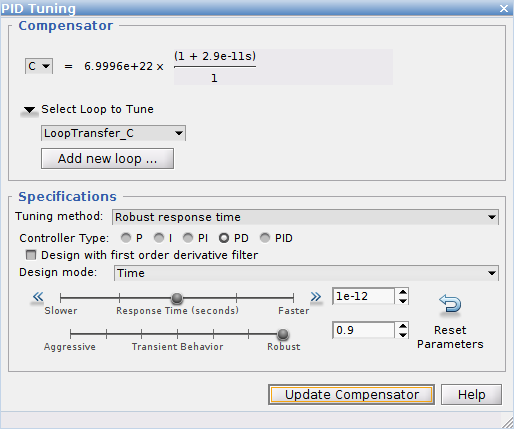
\includegraphics[width=0.5\textwidth]{img/pid_tune.png}
	\caption{}
	\label{fig:pid_tune}
\end{figure}

\end{document}